\chapter{Theoretische Grundlagen}

\section{Sensoren} \label{sensoren:section}

Sensoren sind entscheidend für die 3D Navigation anhand eines externen Umweltmodells. Diese Sensoren werden verwendet, um präzise Informationen über die Umgebung eines Geräts zu erfassen, die dann zur Erstellung des Umweltmodells genutzt werden können. Zu den am häufigsten verwendeten Sensoren gehören Kameras, die RGB- und Tiefeninformationen erfassen, sowie LiDAR-Sensoren, die Entfernungsmessungen durchführen. Diese Sensoren werden in der Robotik, autonomen Fahrzeugen und anderen Anwendungen eingesetzt, um genaue Karten und Modelle der Umgebung zu erstellen, die für eine präzise Navigation erforderlich sind. Die Verwendung von Sensoren ermöglicht es Geräten, ihre Umgebung wahrzunehmen und sich darin zu orientieren, was für eine Vielzahl von Anwendungen von entscheidender Bedeutung ist.

    \subsection{Magnetometer} \label{magnetometer:subsection}

    Bei Magnetometern handelt es sich um Sensoren, die das Magnetfeld im Umfeld des Sensors messen können.
    Diese können sowohl in der Luft, als auch auf dem Boden eingesetzt werden.
    Die Sensoren sind in der Lage, das Magnetfeld in drei Dimensionen zu messen und darzustellen.
    Magnetometrie ist ein wichtiges Instrument in der Navigation, insbesondere in der inertialen Navigation und im autonomen Fahren, wo die genaue Bestimmung der Fahrzeugorientierung entscheidend ist. Es gibt verschiedene Arten von Magnetometern, wie Hall-Sensoren, Fluxgate-Sensoren und Magnetoresistive-Sensoren, die alle auf unterschiedlichen physikalischen Prinzipien basieren. Diese Sensoren können sowohl auf der Erdoberfläche als auch in der Luft eingesetzt werden, um das magnetische Feld zu messen.

    Die Messung des Magnetfeldes erfolgt dabei in der Regel über einen Halbleiter, der durch das Magnetfeld beeinflusst wird und einer Elektronik, die das Signal aufbereitet und ausgibt.
    Magnetometer können jedoch nur die Richtung des Magnetfeldes messen, jedoch nicht die Stärke des Magnetfeldes.
    Magnetometer werden verwendet, um die Ausrichtung von Geräten in bestimmten Koordinatensystemen zu bestimmen.
    Sie können für diese Ausrichtungsbestimmung auch in der Luft verwendet werden. 
    \subsection{Azure Kinect \ac{DK}}

    Das Azure Kinect DK ist ein System, das für die Erfassung von Tiefenbildern und 3D-Modellen eingesetzt wird. Das System besteht aus einer RGB-Kamera und einer Tiefenkamera, die in Kombination arbeiten, um präzise räumliche Tiefeninformationen zu erfassen und 3D-Modelle zu generieren.
    
    \subsubsection{Kamera} \label{kamera:section}
    Eine Kamera ist ein Gerät, das in der Lage ist, visuelle Informationen aufzunehmen und zu speichern. Die Funktionsweise einer Kamera basiert auf der Verwendung von optischen Linsen und einem Bildsensor. Das Licht fällt durch die Linse auf den Bildsensor, der das Licht in elektronische Signale umwandelt, die dann von einem Prozessor verarbeitet und in ein digitales Bild umgewandelt werden. Der Prozessor kann auch Funktionen wie Fokussierung, Belichtung und Weißabgleich steuern. Die resultierenden digitalen Bilder können dann gespeichert oder übertragen werden. 

    Das Azure Kinect \ac{DK} verwendet 2 Kameras, wie in Auflistung \ref{azure-kamera}

    \begin{description}

        \label{azure-kamera}
        \item[RGB Kamera] Die RGB-Kamera des Azure Kinect DK ist eine hochauflösende Farbkamera, die auf einem 1/2.5" CMOS-Sensor basiert. Die Kamera hat eine Auflösung von 3840 x 2160 Pixeln (4K) und verfügt über einen Rolling-Shutter, der die Bildaufnahme zeilenweise abarbeitet, um Bewegungsunschärfe zu reduzieren. Das System ist in der Lage, Farbinformationen und Texturdaten zu erfassen, die für die Erstellung von 3D-Modellen genutzt werden können.
        \item[Depth Kamera] Die Tiefenkamera des Azure Kinect \ac{DK} nutzt einen Time-of-Flight-Sensor, um Tiefenbilder zu erfassen. Die Kamera sendet Infrarot-Licht aus, das vom Objekt reflektiert und von der Kamera empfangen wird. Die Zeit, die das Licht braucht, um zum Objekt und zurück zur Kamera zu gelangen, wird gemessen und zur Berechnung der Entfernung genutzt. Die Auflösung der Tiefenkamera beträgt 1024 x 1024 Pixel, was für eine präzise Erfassung der Tiefeninformationen ausreichend ist. Die Tiefenkamera untersützt verschiedene Modi. Folgende Modi werden unterstützt.
    
    \begin{itemize}
            \item NFOV\_UNBINNED (NFOV): Normaler Sichtbereich, unbinär (ungebündelt) und unverzerrt. Eignet sich für die meisten Anwendungen und liefert eine präzise Tiefenkarte mit hoher räumlicher Auflösung.
            \item NFOV\_BINNED (NFOV): Normaler Sichtbereich, binär (gebündelt) und unverzerrt. Bietet eine höhere Bildrate und eignet sich für Anwendungen, die keine hohe räumliche Auflösung benötigen, wie z.B. Körperverfolgung oder Objekterkennung.
            \item WFOV\_UNBINNED (WFOV): Weitwinkel-Sichtbereich, unbinär und unverzerrt. Bietet eine größere Abdeckung des Sichtbereichs und ist ideal für Anwendungen wie z.B. Umgebungserkennung oder Indoor-Kartierung.
            \item WFOV\_BINNED (WFOV): Weitwinkel-Sichtbereich, binär und unverzerrt. Bietet eine höhere Bildrate und ist nützlich für Anwendungen wie z.B. Körperverfolgung oder Objekterkennung in einem breiteren Sichtbereich.
            \item PASSIVE\_IR (IR): Infrarot-Sichtbereich, binär und unverzerrt. Eignet sich für Anwendungen, bei denen Lichtbedingungen schlecht sind oder Infrarot-Signale genutzt werden, wie z.B. bei der Erfassung von Gesten.
        \end{itemize}
    \end{description}

        
    
        Durch die Kombination von RGB- und Tiefenkamera ist das Azure Kinect \ac{DK} in der Lage, präzise räumliche Tiefeninformationen zu erfassen und 3D-Modelle zu generieren. Das System kann in einer Vielzahl von Anwendungen eingesetzt werden, wie zum Beispiel in der Robotik, virtuellen Realität und Augmented Reality. Es kann auch für die Erfassung von Bewegungen und Gesten genutzt werden, was in der Computergrafik und im Maschinenlernen von Vorteil ist.


        Zusätzlich zur RGB- und Tiefenkamera verfügt das Azure Kinect \ac{DK} auch über eine integrierte Inertial Measurement Unit (\ac{IMU}). Die \ac{IMU} besteht aus einem Beschleunigungsmesser und einem Gyroskop, die Bewegungsdaten erfassen und zur Bestimmung der Orientierung und Position des Geräts im Raum genutzt werden können. Die \ac{IMU} kann auch zur Kompensation von Bewegungsunschärfe und zur Stabilisierung von 3D-Modellen genutzt werden.

\subsubsection{\acl{IMU}}

Das Azure DK (Development Kit) enthält eine integrierte IMU (Inertial Measurement Unit), die aus einem 3-Achsen-Beschleunigungsmesser und einem 3-Achsen-Gyroskop besteht. Die IMU erfasst die Beschleunigung und Rotation des Geräts und liefert entsprechende Daten, die für die Navigation und Stabilisierung verwendet werden können.

Die \ac{IMU} im Azure Kinect \ac{DK} ist speziell darauf ausgelegt, zusammen mit den Kameras des Systems zu arbeiten. Sie ist in der Lage, genaue Daten in Echtzeit zu liefern und kann zur Verbesserung der räumlichen Genauigkeit der Tiefenbilder beitragen. Die IMU kann auch in Kombination mit anderen Sensoren und Systemen genutzt werden, um die Bewegung und Position von Geräten und Robotern in Echtzeit zu verfolgen.
Im Kapitel \ref{chp:slam}\todo{referenz} wird auf die Zusammenarbeit von Kamera und IMU eingegangen.

Insgesamt ermöglicht die Integration einer \ac{IMU} dem Azure Kinect \ac{DK} eine noch präzisere und zuverlässigere Erfassung von Tiefeninformationen und Bewegungsdaten. Dies macht das System zu einem leistungsfähigen Werkzeug für eine Vielzahl von Anwendungen in der Robotik, virtuellen Realität, Augmented Reality und anderen Bereichen, in denen eine genaue räumliche Erfassung erforderlich ist.

        \todo{Quellen}



    

    \subsection{Abstandssensoren} \label{abstandssensoren:subsection}

    Distanzsensoren sind Sensoren, die den Abstand oder die Nähe eines Objekts zu einem anderen Objekt oder einer Oberfläche messen. Es gibt verschiedene Arten von Abstandssensoren, einschließlich Ultraschallsensoren, Infrarotsensoren, Lasersensoren und Laufzeitsensoren. Diese Sensoren werden in verschiedenen Anwendungen eingesetzt, z. B. in der Robotik, in der Automobilindustrie, in der industriellen Automatisierung, in Überwachungssystemen und in Navigationssystemen. Abstandssensoren spielen auch eine wichtige Rolle in der Robotik und Autonomie, insbesondere bei der Umgebungswahrnehmung, Navigation und Hindernisvermeidung. In dieser Studienarbeit werden Depth Kameras und Laser Range Finder für die Abstandsbestimmung verwendet.

    

    \subsubsection{Laser Range Finder}
    Ein Laser-Entfernungsmesser ist ein optoelektronisches Messinstrument, das zur Bestimmung der Entfernung zwischen einem Sender und einem Zielobjekt eingesetzt wird. Das grundlegende Prinzip der Messung beruht auf der Messung der Laufzeit eines ausgesandten Laserpulses, der auf das Zielobjekt trifft und reflektiert wird. Die Laufzeit des Laserpulses wird dann in eine Entfernung umgerechnet.
    Die Messung erfolgt durch das Senden eines kurzen Laserimpulses auf das Zielobjekt, dessen Reflexion vom Empfänger des Entfernungsmessers aufgefangen wird. Die Zeit, die der Laserimpuls benötigt, um das Zielobjekt zu erreichen und zurückzukehren, wird gemessen und in eine Entfernung umgerechnet. Dabei wird die Laufzeit des Laserpulses mit der Lichtgeschwindigkeit multipliziert und durch zwei geteilt, um die Entfernung zum Zielobjekt zu bestimmen.
    \begin{center}
    $Entfernung = \frac{Laufzeit\ des\ Laserimpulses\ x\ Lichtgeschwindigkeit}{2}$
    \end{center}


    \subsubsection{\ac{RGBD} Kameras}
    Infrarot-Tiefenkameras, auch bekannt als RGB-D-Kameras (RGB-Color-Depth), sind optoelektronische Geräte, die zur Erfassung von Bildern verwendet werden und zusätzlich Tiefeninformationen liefern. Diese Kameras arbeiten mit einem optischen System, das einen projizierten Infrarotstrahl auf das zu erfassende Objekt lenkt und mit einer speziellen Kamera dessen Reflexionen erfasst. Auf diese Weise wird eine räumliche Tiefeninformation erstellt, die als Tiefenkarte bezeichnet wird.

    Die Funktionsweise einer Infrarot-Tiefenkamera basiert auf dem Prinzip der Laufzeitmessung (Time-of-Flight, ToF). 
    Es handelt sich dabei um ein Strukturlichtverfahren.
    Dabei wird ein Lichtstrahl von einem Infrarotsender auf ein Objekt projiziert. Das Licht wird von der Oberfläche des Objekts reflektiert und von einem Infrarot-Empfänger in der Kamera aufgefangen. Die Zeit, die das Licht vom Sender zum Empfänger benötigt, wird gemessen und als "Laufzeit" bezeichnet.
    
    Da die Geschwindigkeit des Lichts konstant ist, kann die Entfernung zwischen Kamera und Objekt durch Messung der Flugzeit des Lichtstrahls berechnet werden. Diese Entfernungsinformationen werden in der Tiefenkarte abgebildet. Infrarot-Tiefenkameras können auch Farbinformationen aufnehmen, indem sie eine RGB-Kamera in das System integrieren. Durch die Kombination der Tiefenkarte mit der Farbinformation entsteht ein RGB-D-Bild, das die Form und die Farbe des Objekts in Echtzeit darstellt.

    \subsubsection{Vergleich}\label{chp:depth-sensor-compar}
    Infrarot-Tiefenkameras (RGB-D-Kameras) und Laser-Entfernungsmesser finden auch Anwendung im Bereich der Drohnentechnologie.

Infrarot-Tiefenkameras können beispielsweise in Drohnen eingesetzt werden, um eine präzise Hinderniserkennung und -vermeidung zu ermöglichen. Die Kameras können die räumliche Tiefe von Objekten erfassen und somit eine zuverlässige Entfernungsmessung durchführen. Damit kann die Drohne selbstständig Hindernisse erkennen und ausweichen, was insbesondere in unübersichtlichem Gelände oder in der Indoor-Navigation von Vorteil ist.

ToF-Messungen haben in der Regel eine größere Blickfeldbreite als Laser-Entfernungsmessungen, was bedeutet, dass sie ein größeres Sichtfeld abdecken können. Dies liegt daran, dass ToF-Messungen Infrarotlicht verwenden, das breiter streut als Laserlicht. Dadurch können ToF-Sensoren größere Bereiche in einem einzigen Messvorgang abdecken und somit mehr Inhalte aufnehmen.

Darüber hinaus haben ToF-Sensoren in der Regel auch eine höhere Bildrate als Laser-Entfernungsmesser. Dies bedeutet, dass sie schneller und kontinuierlicher messen können, was für Anwendungen wie Bewegungserkennung und -verfolgung nützlich sein kann.

Laser-Entfernungsmesser werden häufig eingesetzt, um präzise Entfernungen zu messen, wie beispielsweise bei der Vermessung von Land oder Gebäuden. In der Drohnentechnologie können Laser-Entfernungsmesser eingesetzt werden, um präzise Landungen und Abflüge durchzuführen oder um die exakte Position der Drohne zu bestimmen.




\section{ROS - Robot Operating System} \label{ros:section}
In den vergangenen Jahren hat die Wissenschaft im Bereich der Robotik enorme Fortschritte gemacht. Die Verfügbarkeit zuverlässiger und kostengünstiger Roboterhardware, angefangen bei mobilen Bodenrobotern über Quadrotor-Hubschrauber bis hin zu humanoiden Robotern, ist heute größer als jemals zuvor. Noch beeindruckender ist jedoch die Tatsache, dass Algorithmen entwickelt wurden, die diesen Robotern einen immer höheren Grad an Autonomie verleihen.

Trotz dieser rasanten Fortschritte stehen Softwareentwickler jedoch noch immer vor großen Herausforderungen bei der Programmierung von Robotern. Die Komplexität der Aufgaben, die von Robotern ausgeführt werden können, erfordert eine Menge an spezialisiertem Wissen und Erfahrung in verschiedenen Bereichen wie Sensorik, Bildverarbeitung, Künstlicher Intelligenz und Robotik.

Die Igeneure und Softwareentwickler haben jedoch die Herausforderungen erkannt und arbeitet intensiv daran, sie zu lösen. Neue Werkzeuge und Frameworks werden entwickelt, um Entwicklern zu helfen, Roboter schneller und effektiver zu programmieren. Eines der bekanntensten Tools in diesem Bereich ist das Robot Operating System \ac{ROS}

\ac{ROS} ist eine Open-Source-Plattform, die speziell für die Entwicklung von Robotersoftware entwickelt wurde. Es bietet eine Reihe von Bibliotheken, Tools und Frameworks, die es Entwicklern ermöglichen, komplexe Robotikanwendungen zu erstellen und zu betreiben. \ac{ROS} wurde von Willow Garage entwickelt und ist heute ein weit verbreitetes Framework in der Robotik-Community.

\ac{ROS} besteht aus verschiedenen Modulen, die es ermöglichen, Roboterhard-  und software zu abstrahieren und zu standardisieren. Die Plattform bietet eine Vielzahl von Werkzeugen für die Entwicklung von Robotik-Software, einschließlich Visualisierungstools, Datenverarbeitungs- und Analysetools sowie eine umfassende Dokumentation.

\ac{ROS} ist so konzipiert, dass es auf einer Vielzahl von Betriebssystemen und Hardwarearchitekturen laufen kann und bietet Unterstützung für eine breite Palette von Robotern und Sensoren. Es ist auch bekannt für seine Fähigkeit zur Zusammenarbeit zwischen verschiedenen Robotern, die miteinander kommunizieren und Aufgaben gemeinsam erledigen können.

Dank seiner leistungsstarken Funktionen und Flexibilität ist \ac{ROS} zu einem der wichtigsten Frameworks für die Robotik-Entwicklung geworden und wird in vielen Anwendungen eingesetzt, von industriellen Robotern bis hin zu autonomen Fahrzeugen.

    \subsection{Vorraussetzungen zur Verwendung von ROS} \label{Vorraussetzungen zur Verwendung von ROS:subsection}
    \ac{ROS} kann man nicht auf jedem Betriebssystem verwenden. Lauffähig ist es nur auf Unix basierenden Systemen. Am besten funktioniert hierbei Linux und hierbei Ubuntu. Aber auch auf Mac OS kann man ROS verwenden. Allerdings ist die Version für Mac OS bislange nur experimentell. Unter Microsoft Windows direkt kann \ac{ROS} nicht verwenden. Allerdings kann man durch die Verwendung von Docker oder einer virtuellen Maschiene mit z.B. Linux als Gastsystem auch von Windows Computern \ac{ROS} verwenden \cite[vgl.][]{ROS_Introduction}.

    Die \ac{ROS} Version, welche für diese Arbeit verwendet wurde, ist die Version "ROS Noetic Ninjemys". Diese ist die neuste ROS 1 Version mit long term support. Das Betriebssystem, auf welches die Version abzielt, ist Ubuntu 20.04 (Focal). Dementsprechend wurde auch Ubuntu 20.04 für diese Arbeit verwendet.

    \subsection{Ebenen von ROS} \label{Ebenen von ROS:subsection}
    Wie in \cite{ROS_concepts}

    \subsection{ROS-Distributionen} \label{ROS-Distributionen:subsection}
    Eine ROS-Distribution besteht aus einem festgelegten und visionierten Set von ROS-Paketen. Vergelichbar ist dieses System mit den Linux-Distributionen wie z.B. Ubuntu. Der Hauptzweck von ROS-Distributionen besteht darin, Entwicklern eine relativ stabile Codebasis zu bieten, damit sie daran weiterarbeiten können. Sobald eine Distribution veröffentlicht wurde, werden Änderungen hauptsächlich auf Fehlerbehebungen und nicht-zerstörerische Verbesserungen für die Kernpakete (alles unter ros-desktop-full) beschränkt. Somit ist das "Umziehen" auf eine neue Distribution weniger Fehleranfällig und einfacher. Dies gilt im Allgemeinen für die gesamte ROS-Community, jedoch sind die Regeln für "höhere" Pakete weniger streng und somit liegt es an den Verantwortlichen eines spezifischen Pakets, zerstörende Änderungen zu vermeiden \cite[vgl.][]{ROS_contributions}.

    \subsection{Nodes} \label{nodes:subsection}
    In \ac{ROS} werden Funktionen und Prozesse durch sogenannte Nodes realisiert. Eine Node ist eine ausführbare Einheit, die in einem \ac{ROS}-System arbeitet und über eine eindeutige Identifikation verfügt. Jede Node hat eine spezifische Aufgabe, wie beispielsweise das Sammeln von Sensordaten, die Ausführung einer spezifischen Berechnung oder das Steuern eines Aktors.

    Nodes können miteinander kommunizieren, indem sie Nachrichten senden und empfangen. Nachrichten sind definierte Datenstrukturen, die Informationen zwischen Nodes transportieren. Nodes können auch Services anbieten oder anfordern, um eine bestimmte Aktion auszuführen.

    Eine wichtige Funktion von Nodes ist ihre Fähigkeit zur Verteilung. In \ac{ROS} können Nodes auf verschiedenen Hosts oder in verschiedenen Prozessen ausgeführt werden. Dadurch können komplexe \ac{ROS}-Systeme erstellt werden, die aus vielen miteinander verbundenen Nodes bestehen.

    Nodes können auch in einer \ac{ROS}-Graphenstruktur organisiert werden. Diese Struktur zeigt die Abhängigkeiten zwischen Nodes und die Art der Kommunikation zwischen ihnen an. Die \ac{ROS}-Graphenstruktur kann mit Werkzeugen wie "rqt\_graph" visualisiert werden, um eine bessere Übersicht über das System zu erhalten.

    Die Verwendung von Nodes in \ac{ROS} ermöglicht eine hohe Flexibilität und Modularität bei der Entwicklung von Robotik-Anwendungen. Entwickler können einzelne Nodes erstellen, testen und optimieren, bevor sie sie in einem größeren System einsetzen. Darüber hinaus können Nodes wiederverwendet werden, um ähnliche Funktionen in verschiedenen Anwendungen auszuführen.

    Insgesamt sind Nodes eine zentrale Komponente von \ac{ROS} und ermöglichen es Entwicklern, komplexe Roboteranwendungen mit einer hohen Flexibilität und Modularität zu erstellen.

    \subsection{Topics} \label{topics:subsection}
    In \ac{ROS} werden Daten zwischen Nodes durch sogenannte Topics ausgetauscht. Ein Topic ist eine benannte Kommunikationsleitung, über die Nodes Nachrichten senden und empfangen können. Topics ermöglichen die einfache und flexible Kommunikation zwischen Nodes, ohne dass die Nodes über die genaue Identität des Empfängers Bescheid wissen müssen.

    Ein Topic hat einen bestimmten Datentyp, der definiert, welche Art von Daten zwischen Nodes ausgetauscht werden können. Es können beispielsweise Sensordaten wie Bilder oder Entfernungsmessungen, oder Steuerbefehle für Aktoren wie Motoren oder Greifer übertragen werden.

    Nodes können sich auf ein Topic abonnieren, um die Nachrichten, die auf diesem Topic veröffentlicht werden, zu empfangen. Jedes Mal, wenn eine Nachricht auf einem Topic veröffentlicht wird, wird sie an alle Nodes weitergeleitet, die auf dieses Topic abonniert sind.

    Topics können auch von Nodes veröffentlicht werden, um Nachrichten an andere Nodes zu senden. Eine Node, die ein Topic veröffentlicht, wird als Publisher bezeichnet. Der Publisher kann regelmäßig Nachrichten auf einem Topic veröffentlichen, um andere Nodes über Änderungen in der Umgebung oder im System zu informieren.

    Die Verwendung von Topics in \ac{ROS} ermöglicht eine einfache und flexible Kommunikation zwischen Nodes, was besonders in komplexen Systemen von Vorteil ist. Nodes können sich auf mehrere Topics abonnieren und Nachrichten an mehrere Topics veröffentlichen, was eine effektive und modulare Datenverarbeitung ermöglicht. Zudem können Topics auf mehreren Hosts oder in verschiedenen Prozessen ausgeführt werden, was eine Skalierung des \ac{ROS}-Systems ermöglicht.

    Insgesamt sind Topics eine wichtige Komponente von \ac{ROS} und ermöglichen es Entwicklern, eine einfache und effektive Kommunikation zwischen Nodes in Robotik-Anwendungen zu realisieren.

    \subsection{Messages} \label{messages:subsection}
    Die Messages sind Datenströme, die zwischen mindestens zwei Nodes ausgetauscht werden. Sie werden in sogenannten msg-Dateien definiert. Diese Nachrichten können sowohl aus primitiven Datentypen als auch aus Datenstrukturen bestehen. Der Datenfluss erfolgt immer nur in eine Richtung.

    \subsection{Publish and Subscripe Pattern} \label{publish_and_subscripe_pattern:subsection}
    Das Publish-Subscribe-Pattern ist ein grundlegendes Muster der \ac{ROS}-Kommunikation und ermöglicht eine effektive und modulare Datenverarbeitung in verteilten Systemen.

    Beim Publish-Subscribe-Pattern senden Nodes, die Informationen über eine bestimmte Ressource verarbeiten, die Informationen an ein Topic, das als Vermittler dient. Nodes, die an den Informationen interessiert sind, abonnieren das Topic und erhalten alle zukünftigen Nachrichten, die von Nodes veröffentlicht werden, die mit dem Topic verbunden sind.

    Dieses Muster hat mehrere Vorteile. Zum einen ermöglicht es eine flexible Architektur, in der Nodes unabhängig voneinander arbeiten und sich auf das Abonnieren und Veröffentlichen von Topics konzentrieren können, ohne die genaue Identität des Empfängers oder Senders zu kennen. Zum anderen ermöglicht es eine effektive Datenverarbeitung, da mehrere Nodes dieselben Informationen von einem Publisher erhalten können.

    Ein weiterer Vorteil des Publish-Subscribe-Patterns ist, dass es eine einfache Möglichkeit bietet, den Zustand von Ressourcen zu überwachen oder auf Änderungen in Echtzeit zu reagieren. So kann beispielsweise eine Node, die eine Kamera überwacht, die Bilder auf einem Topic veröffentlichen. Andere Nodes, die an der Verarbeitung dieser Bilder beteiligt sind, können sich auf das Topic abonnieren und die Informationen in Echtzeit verarbeiten.

    Das Publish-Subscribe-Pattern ist ein grundlegendes Konzept in \ac{ROS} und wird in der Regel für die Kommunikation zwischen Nodes verwendet. Es ermöglicht eine effektive und modulare Datenverarbeitung in verteilten Systemen und ist ein wesentlicher Bestandteil von \ac{ROS}, um komplexe Robotik-Anwendungen zu realisieren.

    \subsection{Objekterkennung} \label{objekterkennung:subsection}
    In \ac{ROS} gibt es verschiedene Methoden zur Objekterkennung, die in Robotik-Anwendungen eingesetzt werden können. Die Objekterkennung ist ein wichtiger Schritt in der automatisierten Wahrnehmung von Robotern, da sie es ihnen ermöglicht, ihre Umgebung zu verstehen und darauf zu reagieren.

    Eine häufig verwendete Methode zur Objekterkennung in \ac{ROS} ist die Verwendung von 3D-Sensoren wie Lidar oder Kinect. Diese Sensoren erfassen Daten über die Umgebung des Roboters und können dabei helfen, Objekte zu identifizieren und ihre Position und Orientierung im Raum zu bestimmen.
    \todo{Kinect kein Sensor System}
    Eine weitere Methode zur Objekterkennung in \ac{ROS} ist die Verwendung von Bildverarbeitungs-Algorithmen. Dabei können beispielsweise Farb- oder Formmerkmale verwendet werden, um Objekte in Bildern zu erkennen und ihre Position und Ausrichtung zu bestimmen.

    Eine weiterentwickelte Methode zur Objekterkennung in \ac{ROS} ist die Verwendung von Deep-Learning-Methoden wie Convolutional Neural Networks (CNNs). Dabei werden CNNs trainiert, um Objekte in Bildern oder Punktwolken zu erkennen und zu klassifizieren. Diese Methode erfordert jedoch ein umfangreiches Training und eine hohe Rechenleistung, um in Echtzeit ausgeführt zu werden.

    Die Objekterkennung ist ein wichtiger Schritt in der automatisierten Wahrnehmung von Robotern, da sie es ihnen ermöglicht, ihre Umgebung zu verstehen und darauf zu reagieren. \ac{ROS} bietet verschiedene Methoden zur Objekterkennung, die in Robotik-Anwendungen eingesetzt werden können. Die Wahl der richtigen Methode hängt von den Anforderungen der Anwendung ab und erfordert oft eine sorgfältige Abwägung zwischen Genauigkeit, Geschwindigkeit und Komplexität.

    \subsection{QR-Codes} \label{qr-codes:subsection}
    \ac{ROS} bietet verschiedene Möglichkeiten zur Erkennung von QR-Codes in Robotik-Anwendungen. QR-Codes sind zweidimensionale Barcodes, die Informationen wie URLs, Texte oder andere Daten enthalten können. Die Erkennung von QR-Codes kann in \ac{ROS}-basierten Anwendungen genutzt werden, um Informationen zu lesen, Roboter zu navigieren oder um eine Interaktion mit der Umgebung zu ermöglichen.

    Es gibt verschiedene \ac{ROS}-Pakete, die die QR-Code-Erkennung erleichtern. Ein Beispiel ist das "zbar\_ros" Paket, das ein Wrapper für die Open-Source-ZBar-Bibliothek ist, die QR-Codes und andere Barcodes erkennt. Das zbar\_ros-Paket ermöglicht es, den Inhalt von QR-Codes aus dem Kamerabild zu extrahieren und als \ac{ROS}-Topic zu veröffentlichen, der von anderen Nodes abonniert werden kann. Das Paket bietet auch Optionen zur Konfiguration der QR-Code-Erkennung, wie beispielsweise die Festlegung der Mindestgröße des Codes oder die Einstellung der Scan-Frequenz.

    Ein weiteres \ac{ROS}-Paket, das die QR-Code-Erkennung erleichtert, ist das "ros\_qr\_detector" Paket. Dieses Paket basiert auf der OpenCV-Bibliothek und bietet eine einfache Möglichkeit, QR-Codes in \ac{ROS}-basierten Anwendungen zu erkennen. Das Paket bietet auch die Möglichkeit, QR-Codes aus der Kamerabildanzeige auszuschneiden und als separate Bilder zu speichern.

    Die Erkennung von QR-Codes in \ac{ROS}-Anwendungen kann für verschiedene Anwendungsfälle nützlich sein. Beispielsweise können QR-Codes als Marker verwendet werden

    \subsection{Starten eines ROS Programms} \label{starten eines ROS Programms:subsection}
    Zum Starten verschiedener Nodes in \ac{ROS} wird das ROS-eigene Tool roslaunch verwendet. Roslaunch ist ein mächtiges Werkzeug für die Konfiguration, das Starten und die Überwachung von ROS-Paketen und -Nodes. Mit roslaunch können Entwickler schnell und einfach Nodes starten, indem sie eine XML-Datei erstellen, die alle notwendigen Konfigurationen enthält. Die XML-Datei wird als Launch-Datei bezeichnet und wird in der Regel von Entwicklern erstellt, um eine oder mehrere ROS-Knoten gleichzeitig zu starten und zu konfigurieren.

    Ein großer Vorteil von roslaunch ist seine Portabilität. Mit Launch-Dateien können Entwickler ROS-Pakete und -Nodes problemlos auf verschiedenen Systemen starten und konfigurieren, unabhängig von der Plattform oder Architektur. Dies erleichtert die Entwicklung von ROS-Software für verschiedene Roboter- und Hardware-Plattformen erheblich. \cite{roslaunch}

    Der Befehl, mit welchem man roslauch aufruft, sieht wie folgt aus:
    
    \textit{\$ roslaunch package\_name file.launch}

\section{Drohne/Multicopter} \label{drohne:section}
Bei der für das Projekt verwendete Drohne handelt es sich um eine Coex Clover Drohne in der Version Clover 4.2. Dies ist eine programmierbare Drohne, die besonders für Bildungszwecke eingesetzt wird. Sie ist sowohl für den Einsatz draußen sowie auch in Gebäuden geeignet. \\

\begin{figure}[htpb]
    \centering
    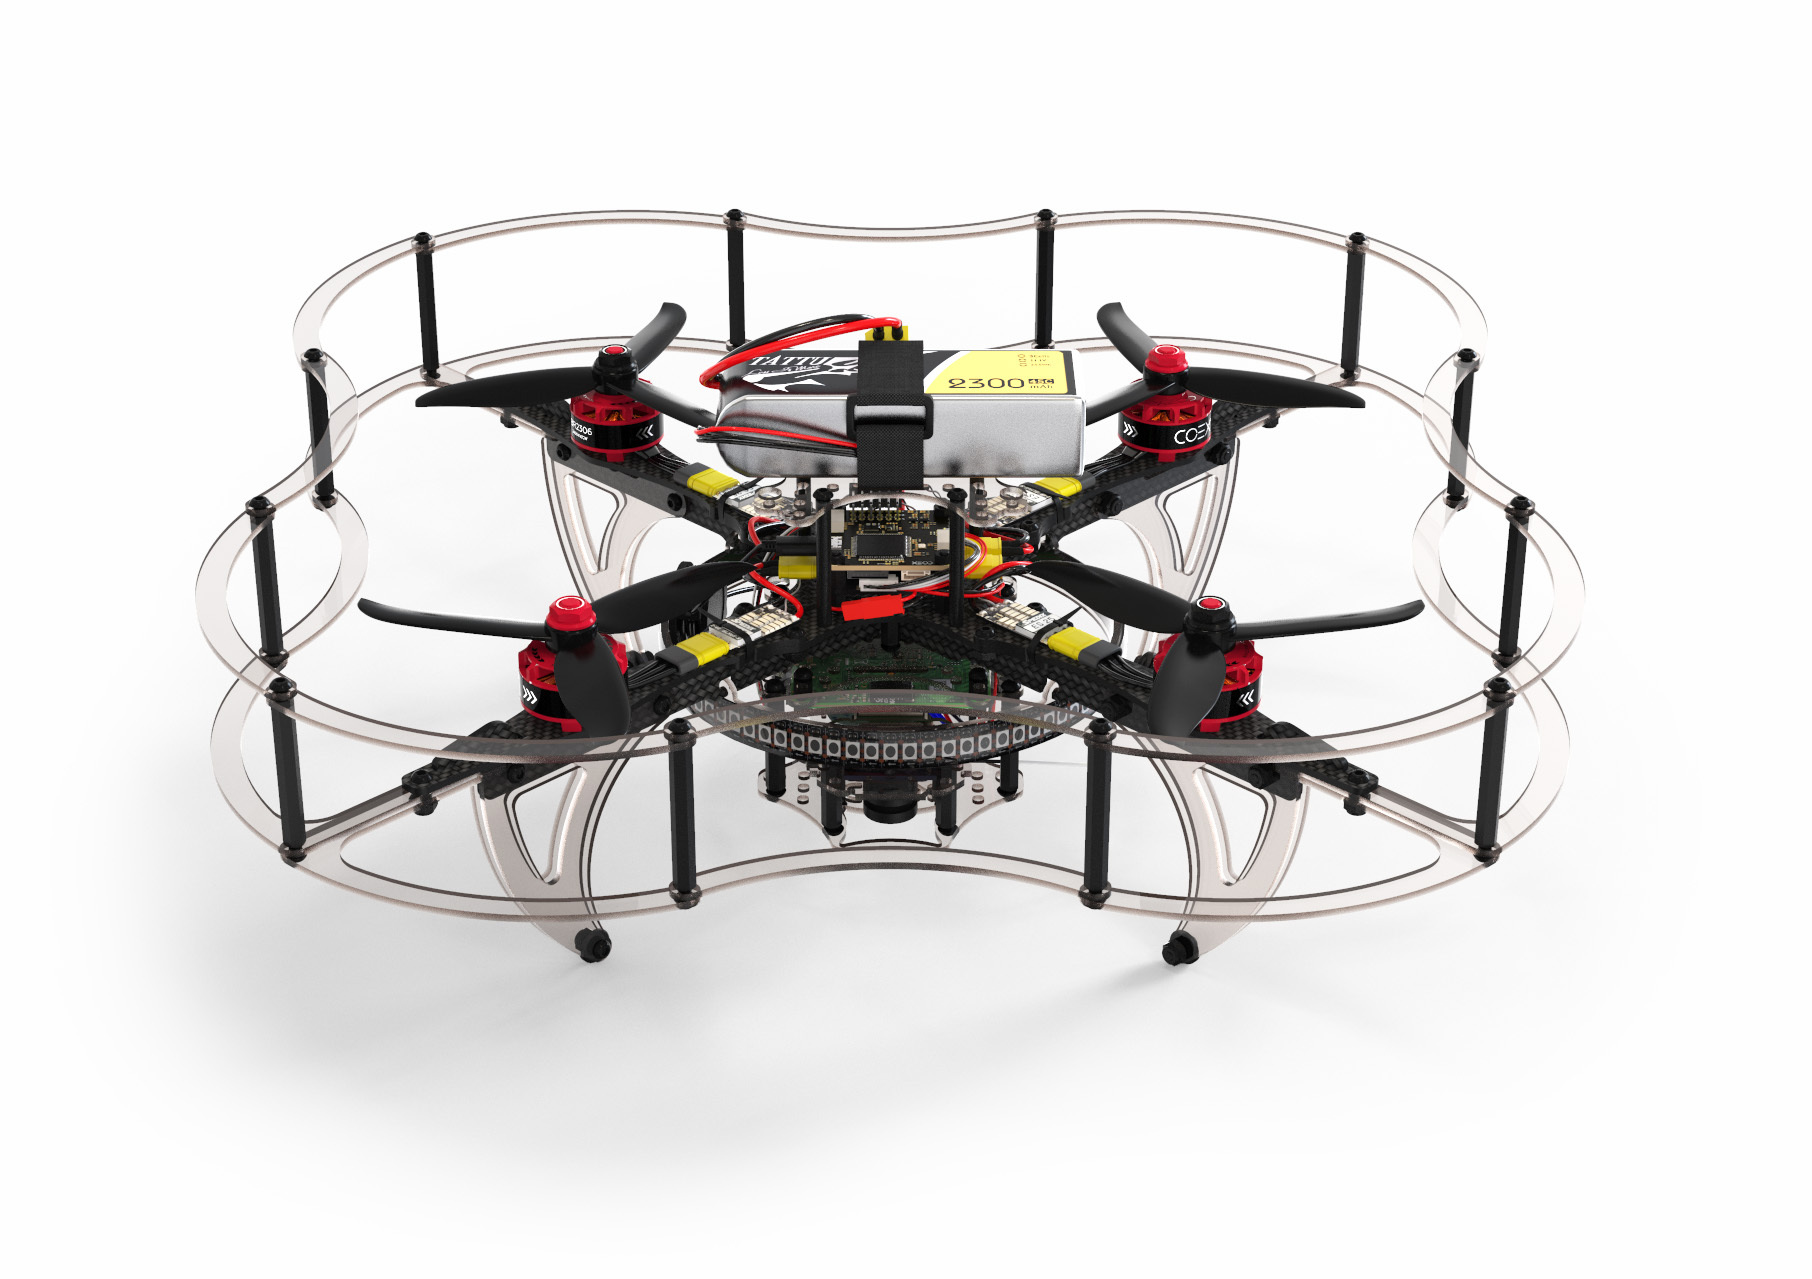
\includegraphics[width=10cm,keepaspectratio,angle=0]{images/coex_clover.jpg}
    \caption[Coex Clover Drohne]{\label{img coex_clover} Coex Clover Drohne \cite{img_coex_clover}}
\end{figure}


Zu Beginn erhält man hierbei einen Bausatz, welcher dann zu einem Quadrokopter zusammengebaut werden kann. Der Vorteil hierbei ist zudem, dass die gesamte Drohne ohne Löten zusammengesetzt werden kann. Zu den einzelnen Bestandteilen der Drohne kommen, noch eine Dokumentation sowie verschiedene Bibliotheken, die es ermöglichen, die Drohne zusammen bauen und fliegen lassen zu können. \\
Durch die Verwendung verschiedener Open-Source Komponenten lässt sich die Drohne programmieren, wodurch ein vielseitiger Einsatzbereich entsteht.\\

\begin{figure}[htpb]
    \centering
    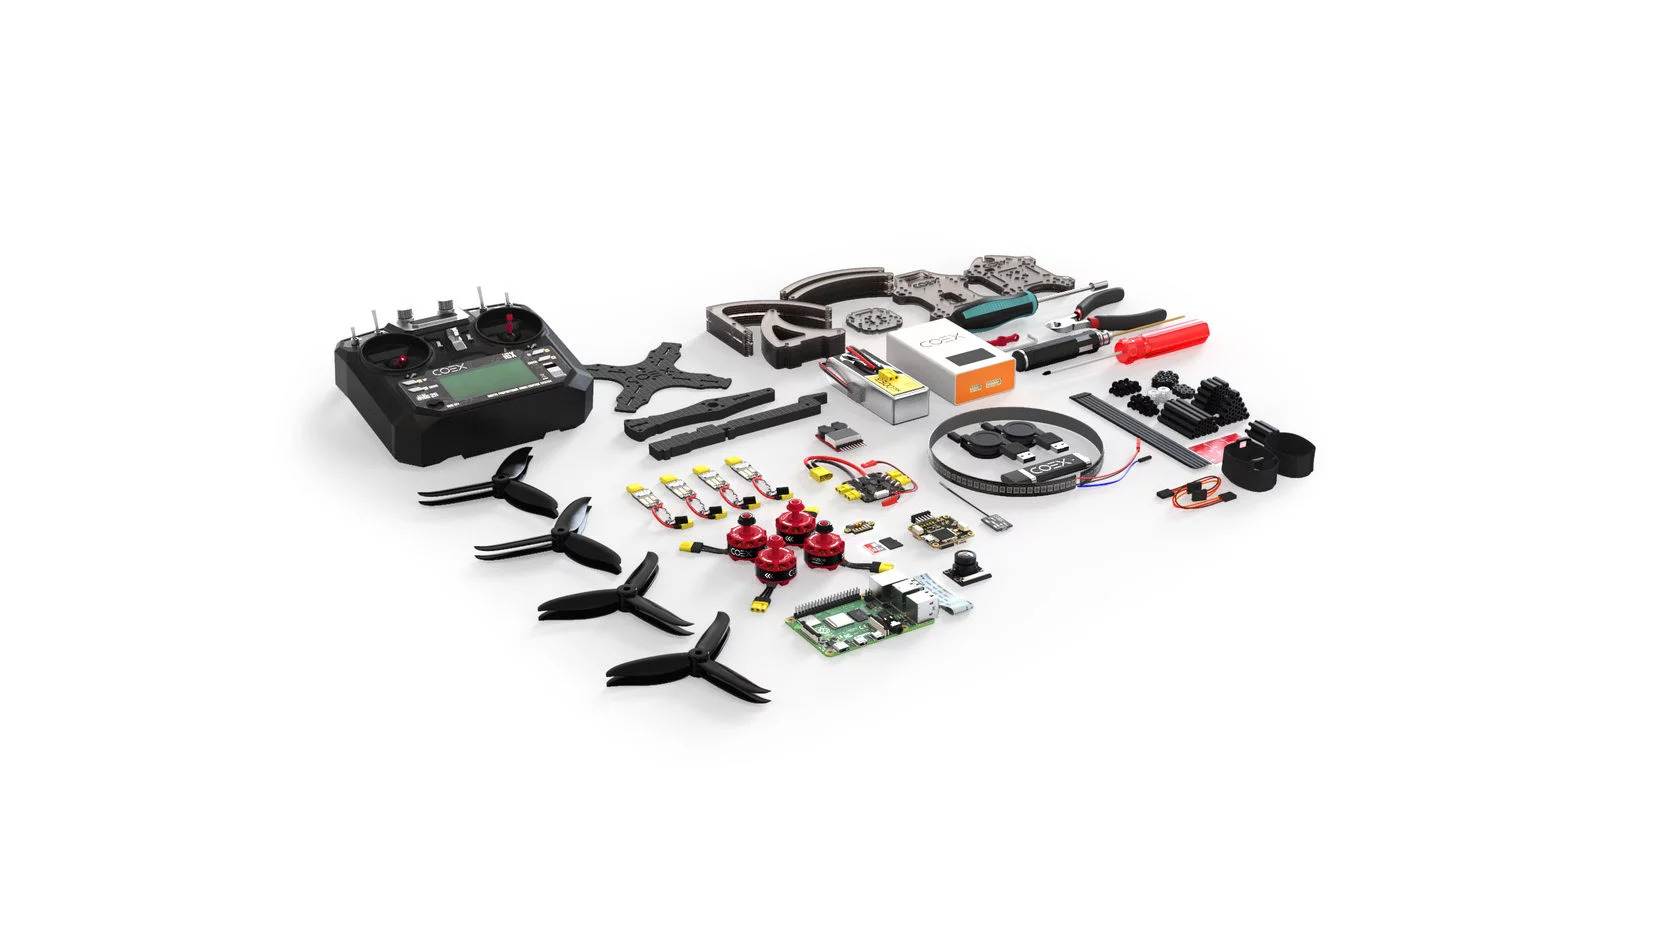
\includegraphics[width=10cm,keepaspectratio,angle=0]{images/coex_clover_kit.jpg}
    \caption[Bausatz Coex Clover Drohne]{\label{img coex_clover_kit} Bausatz Coex Clover Drohne \cite{img_coex_clover_kit}}
\end{figure}

Die Coex Clover Drohne soll laut Herstellerinformationen bis zu 15 Minuten am Stück fliegen können und in dieser Zeit eine Maximalhöhe von 500 Metern bei einer Höchstgeschwindigkeit von bis zu 72 km/h erreichen können \cite[vgl.][]{coex_clover}.\\

Zu den Hauptbestandteilen der Drohne zählen zum einen ein Raspberry Pi 4 sowie der Flightcontroller Coex Pix. Diese bilden die Grundlage zur Programmierung und Steuerung der Coex Clover Drohne und ermöglichen es zudem die Drohne über drahtlos per WLAN zu verbinden. \\
Die Drohne ist ein Quadrokopter und besitzt somit vier Motoren, welche einzeln angesteuert werden können. Sie besitzt zudem eine Vielzahl verschiedener Sensoren, auf welche in Kapitel \ref{sensoren:section} genauer eingegangen wird. Zu diesen zählen unter anderem ein Gyroskop, Magnetometer sowie ein Laseranstandssensor und eine Kamera, die unten an der Drohne angebracht sind.
Zum Schutz befindet sich zudem außen einen Rahmen.
Bei der Drohne war zudem ein 2300 mAh großer Akku dabei, der für vom Hersteller angegebene Flugdauer sorgen soll.
Im Folgenden wird nun auf die wichtigsten Bestandteile der Coex Clover Drohne noch einmal genauer eingegangen:

\subsection{Raspberry Pi 4} \label{raspberry_pi:subsection}

Die Coex Clover Drohne, welche für diese Arbeit genutzt wurde, enthält einen Raspberry Pi 4 Model B mit 1 GB Arbeitsspeicher.\\
Der Raspberry Pi beinhaltet zudem eine austauschbare MicroSD-Karte, auf welche sich in diesem Fall das Raspberry Pi Betriebssysteme befindet. \\

\begin{figure}[htbp]
    \centering
    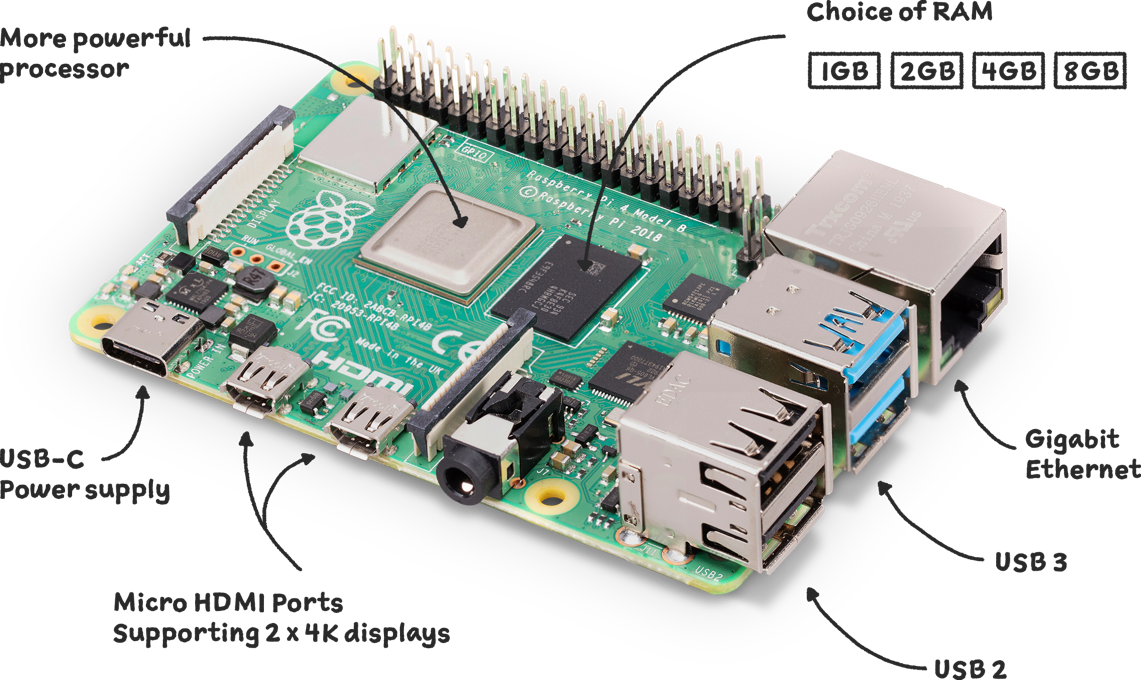
\includegraphics[width=10cm,keepaspectratio,angle=0]{images/raspberry-pi-4-labelled.png}
    \caption[Raspberry Pi 4]{\label{img raspberry_pi} Raspberry Pi 4 \cite{img_raspberry_pi}}
\end{figure}

% sets barrier between this subsections so the picture is above the next subsection
\FloatBarrier

\subsection{Coex Pix} \label{coex_pix:subsection}
Der Coex Pix Flight Controller wird für den Betrieb von Drohnen und anderen Fluggeräten verwendet werden. Hierbei basiert dieser auf der PX4 Software. Der Flight Controller einhaltet verschiedene Sensoren, hierzu gehören ein Accelerometer, Gyroskop und ein Magnetometer.

\todo{Benennung FlightController/FlugController/...}


\subsubsection{PX4} \label{px4:subsection}
PX 4 ist eine Open-Source-Software, welche zur Steuerung verschiedener Arten von Fahrzeugen genutzt werden kann, hierzu zählen beispielsweise verschedne Drohenarten, sowie auch Fahrzeuge auf dem Boden und Unterwasserfahrzeuge.\\ Es kann zum einen für bereits flugfähigen Drohen einesetztwerden. Aber es besteht auch die Möglichkeit eine neue Drohne in Verbindung mit PX4 zu bauen.\\
Für die Verwendung der PX4 Software kann QGroundControl (siehe Kapitel \ref{qGroundControl:subsection}) verwendet werden. \cite[vgl.][]{px4} \\
Der PX4-Flugstack wurde ursprünglich nur dür die Pixhawk-Hardware entwickelt, allerdings ist es heutzutage auch möglich diesen auf Linux-Computern und anderen Hardware einzusetzen. Wie es auch bei der Coex Clover Drohne mit dem Coex Pix umgesetzt wird. \\
Die Software setzt Sensoren, ein um den Zustand der Drohne zu bestimmen. Hierfür werden einige Sensoren vorrausgesetzt, zu diesen zählen ein Gyroskop, ein Beschleunigungssensor, ein Magnetometer sowie ein Barometer. Zudem ist GPS empfohlen um weitere Modis nutzen zu können. \cite[vgl.][]{px4}

\subsubsection{QGroundControl}  \label{qGroundControl:subsection}
QGroundControl ist eine Software, welche vor allem für Drohnen mit einem PX4 aber auch anderen Flight Controller genutzt werden kann. Hierbei bietet es verschiedene Funktionen. Zum einen gehört hierzu die Konfiguration der einzelnen  Drohnen. Desweiteren ist es möglich mit der Software verschiedene Flugmodi auszuwählen, sowie diese dann auch während des Fluges zu überwachen, beispielweise durch die Anzeige der Flugposition auf einer Karte sowie auch deren Geschwindigkeit und andere Sensordaten.
Es ist auch möglich mit QGRoudnControl eine ganze Flugplanung zu machen, welche die Drohne daraufhi umsetzt. \cite[vgl.][]{qGroundControl}

\section{3D-Modelle} \label{3d-modelle:section}

\subsection{Punktwolken}
Eine Punktwolke ist eine räumliche Darstellung eines Objekts oder einer Szene in Form einer Sammlung von 3D-Koordinaten. Am Beispiel von \ac{RGBD} Kameras, erfasst eine Punktwolke sowohl Farb als auch Tiefeninformationen aus einer Szene.
Die Tiefeninformationen werden verwendet, um die räumliche Geometrie der Szene zu erfassen und eine Punktwolke zu erstellen.
Die Punktwolke besteht aus einer Sammlung von Punkten, die jeweils eine Position im dreidimensionalen Raum repräsentieren. Jeder Punkt hat in der Regel drei Koordinaten (x, y, z), die seine Position im Raum beschreiben. Die Farbinformationen werden häufig als RGB-Werte (rot, grün, blau) oder als Grauwerte für jeden Punkt in der Punktwolke gespeichert.
Eine RGBD-Kamera erfasst die Tiefeninformationen durch die Verwendung eines Strukturlichtverfahrens oder eines Zeitflugverfahrens. Strukturlichtverfahren arbeiten durch die Projektion von Lichtmuster auf die Szene und das Erfassen der Verzerrungen im Muster, um die Tiefeninformationen zu berechnen. Zeitflugverfahren funktionieren durch die Messung der Zeit, die benötigt wird, um ein Lichtsignal auszusenden und das reflektierte Signal wieder zu empfangen, um die Entfernung und damit die Tiefeninformationen zu berechnen.

Die erfasste Punktwolke wird dann für verschiedene Anwendungen verwendet, wie z.B. für die Erstellung von 3D-Modellen, für die Positionsbestimmung von Robotern oder für die Objekterkennung in der Robotik. Da die Punktwolken alle Informationen über die räumliche Geometrie einer Szene enthalten, sind sie ein wichtiges Instrument für viele Anwendungen in der Robotik, der Computer Vision und der Augmented Reality.


\section{Positionsbestimmung}
Positionsbestimmung ist ein wichtiges Thema in vielen Bereichen, wie der Robotik, autonomem Fahren, Navigation und Augmented Reality. Eine der Herausforderungen bei der Positionsbestimmung ist die Erstellung einer genauen Karte der Umgebung, die es dem mobilen Gerät ermöglicht, seine Position darin zu bestimmen. Hier kommen Technologien wie SLAM (Simultaneous Localization and Mapping) und Spatial Mapping zum Einsatz. Beide Ansätze ermöglichen die Erstellung von 3D-Karten der Umgebung, aber sie unterscheiden sich in ihren Methoden und Anwendungen. In dieser Hinsicht sind SLAM und Spatial Mapping wichtige Technologien für die Positionsbestimmung und haben eine breite Anwendung in verschiedenen Branchen gefunden.

   
    \subsection{Inertielle Positionsbestimmung} \label{inertielle_positionsbestimmung:subsection}
    Inertiale Positionsbestimmung ist ein weiterer Ansatz zur Positionsbestimmung, der auf der Verwendung von Inertialsensoren wie Gyroskopen und Beschleunigungsmessern basiert. Inertialsensoren messen die Veränderungen der Beschleunigung und der Winkelgeschwindigkeit eines mobilen Geräts, was dazu verwendet werden kann, die Position und Orientierung des Geräts in der Umgebung zu bestimmen. Im Gegensatz zu SLAM und Spatial Mapping benötigt die inertielle Positionsbestimmung keine 3D-Karte der Umgebung und ist daher in der Lage, in Echtzeit eine präzise Positionsbestimmung durchzuführen.

Allerdings ist die inertielle Positionsbestimmung anfällig für Fehler, die aufgrund von Drift und Ungenauigkeiten der Inertialsensoren entstehen können. Um diese Fehler zu minimieren, wird die inertielle Positionsbestimmung oft mit anderen Technologien wie GPS oder visuellen Systemen kombiniert. Diese Kombination von Technologien wird auch als Sensorfusion bezeichnet und ermöglicht eine präzisere und robustere Positionsbestimmung in verschiedenen Anwendungen wie Drohnen, autonomen Fahrzeugen und Wearables.
\subsection{SLAM} \label{SLAM:section} \label{positionsbestimmung:section}
Der SLAM-Prozess umfasst die simultane Bestimmung der Position eines mobilen Geräts in der Umgebung und die Erstellung einer Karte dieser Umgebung. Dies wird durch die Integration von Daten aus verschiedenen Sensoren wie Kameras, Inertialsensoren und Entfernungsmessern wie Laser-Scannern oder Time-of-Flight-Sensoren erreicht. Der SLAM-Prozess wird oft in der Robotik und in autonomen Fahrzeugen eingesetzt, um eine präzise Karte der Umgebung zu erstellen und sich gleichzeitig darin zu lokalisieren.
Durch die Kombination der Inertialsensoren mit anderen Sensoren kann eine präzisere und robustere Positionsbestimmung erreicht werden, indem die Vorteile der verschiedenen Technologien kombiniert werden. Die Inertialsensoren können beispielsweise verwendet werden, um die Bewegung des mobilen Geräts zwischen den einzelnen Beobachtungen durch die anderen Sensoren zu messen und die Positions- und Orientierungsdaten der SLAM-Systeme zu korrigieren.

Ein SLAM System besteht aus verschiedenen Teilsystemen.

\subsubsection{Punktwolkengeneration}
Ein Punktwolkengenerator erzeugt eine Punktwolke aus mehreren Bildern, die von einer Kamera aufgenommen wurden. Zunächst wird die intrinsische Matrix der Kamera benötigt, um die 2D-Bildpunkte in eine korrekte 3D-Repräsentation umzuwandeln. Diese Matrix beschreibt die Abbildungseigenschaften der Kamera und enthält Informationen wie Brennweite, Verschiebung und Verzerrung. Um diese Matrix zu erhalten, werden Kalibrierungsbilder von der Kamera aufgenommen und anschließend eine Kalibrierungssoftware verwendet, um die intrinsischen Parameter der Kamera zu berechnen. Sobald die intrinsische Matrix bekannt ist, kann die extrinsische Matrix bestimmt werden. Diese Matrix beschreibt die Position und Ausrichtung der Kamera im Raum relativ zum Weltkoordinatensystem. Um diese Matrix zu berechnen, werden mehrere Bilder von der Kamera aus verschiedenen Positionen aufgenommen und mithilfe von visuellen Odometrie- oder SLAM-Algorithmen verarbeitet, um die Kameraposition und -orientierung zu schätzen.Nachdem die intrinsischen und extrinsischen Matrizen bekannt sind, können die 2D-Bildpunkte in 3D-Objektpunkte umgewandelt werden. Dies geschieht durch die Rückprojektion von jedem 2D-Bildpunkt in den Raum entlang der Sichtlinie der Kamera. Die Position und Orientierung der Kamera sowie die intrinsischen Parameter bestimmen den Punkt, an dem die Sichtlinie des 2D-Punktes die 3D-Szene schneidet.

Durch Wiederholung dieses Prozesses für jedes 2D-Bild wird eine Punktwolke erzeugt, die eine dreidimensionale Repräsentation der Szene darstellt. Die resultierende Punktwolke kann für verschiedene Anwendungen wie 3D-Rekonstruktion, Objekterkennung und Augmented Reality verwendet werden.








\subsection{Spatial Mapping} \label{spatial_mapping:subsection}
Spatial Mapping hingegen ist ein Prozess, bei dem eine 3D-Karte der Umgebung auf der Grundlage der Verarbeitung von Kameradaten erstellt wird. Im Gegensatz zum SLAM-Prozess muss das mobile Gerät, das die 3D-Karte erstellt, seine Position in der Umgebung bereits kennen, da es auf der Verarbeitung von Kameradaten basiert. Die Kameras nehmen Bilder auf und wandeln sie in 3D-Punktwolken um, die dann zu einer Karte kombiniert werden. Spatial Mapping wird in Augmented-Reality-Anwendungen und anderen Anwendungen eingesetzt, bei denen eine genaue 3D-Karte der Umgebung benötigt wird.
\section{Regelsysteme} \label{regelsysteme:section}

    \subsection{PID-Regler} \label{pid_regler:subsection}

    \subsection{Extended Kalman Filter 2}
    Der \ac{EKF}2-Algorithmus, der in der Drohnensteuerung verwendet wird, ist eine Erweiterung des klassischen erweiterten Kalman-Filters, die speziell auf die Bedürfnisse der Drohnensteuerung zugeschnitten ist. Der EKF2 ist ein geschätzter Zustandsregler, der die aktuellen Zustände (z.B. Position, Geschwindigkeit, Orientierung) einer Drohne schätzt, basierend auf Messungen von Sensoren (z.B. \ac{GPS}, \ac{IMU}, Magnetometer).

Im Gegensatz zum klassischen EKF verwendet der EKF2 eine modifizierte Version der Kalman-Filter-Formeln, um den Einfluss von Sensorrauschen und Messfehlern besser zu berücksichtigen. Insbesondere verwendet der EKF2 eine sogenannte "Innovation Covariance Matrix", die die Varianz der Messfehler repräsentiert und in die Filtergleichungen eingebaut wird. Diese Innovation Covariance Matrix wird iterativ während des Betriebs des Filters aktualisiert, um den Sensorrauschen und Messfehlern besser gerecht zu werden.

Darüber hinaus verwendet der EKF2 eine modifizierte Version der State Transition Matrix, die die Nichtlinearitäten des Systems besser modellieren kann. Diese modifizierte Matrix wird ebenfalls iterativ während des Filterbetriebs aktualisiert, um den Änderungen im Systemverhalten besser gerecht zu werden.

In der Drohnensteuerung wird der EKF2-Algorithmus verwendet, um die aktuellen Zustände der Drohne (z.B. Position, Geschwindigkeit, Orientierung) in Echtzeit zu schätzen. Diese Schätzungen werden dann verwendet, um die Steuerbefehle der Drohne zu generieren, um sie auf Kurs zu halten und sicher zu navigieren.


\section{Simulationstechnik} \label{simulationstechnik:section}

\section{Problembehebung} \label{problembehebung:section}
